%% Creator: Inkscape inkscape 0.92.2, www.inkscape.org
%% PDF/EPS/PS + LaTeX output extension by Johan Engelen, 2010
%% Accompanies image file 'expb2.eps' (pdf, eps, ps)
%%
%% To include the image in your LaTeX document, write
%%   \input{<filename>.pdf_tex}
%%  instead of
%%   \includegraphics{<filename>.pdf}
%% To scale the image, write
%%   \def\svgwidth{<desired width>}
%%   \input{<filename>.pdf_tex}
%%  instead of
%%   \includegraphics[width=<desired width>]{<filename>.pdf}
%%
%% Images with a different path to the parent latex file can
%% be accessed with the `import' package (which may need to be
%% installed) using
%%   \usepackage{import}
%% in the preamble, and then including the image with
%%   \import{<path to file>}{<filename>.pdf_tex}
%% Alternatively, one can specify
%%   \graphicspath{{<path to file>/}}
%% 
%% For more information, please see info/svg-inkscape on CTAN:
%%   http://tug.ctan.org/tex-archive/info/svg-inkscape
%%
\begingroup%
  \makeatletter%
  \providecommand\color[2][]{%
    \errmessage{(Inkscape) Color is used for the text in Inkscape, but the package 'color.sty' is not loaded}%
    \renewcommand\color[2][]{}%
  }%
  \providecommand\transparent[1]{%
    \errmessage{(Inkscape) Transparency is used (non-zero) for the text in Inkscape, but the package 'transparent.sty' is not loaded}%
    \renewcommand\transparent[1]{}%
  }%
  \providecommand\rotatebox[2]{#2}%
  \ifx\svgwidth\undefined%
    \setlength{\unitlength}{683.9999829bp}%
    \ifx\svgscale\undefined%
      \relax%
    \else%
      \setlength{\unitlength}{\unitlength * \real{\svgscale}}%
    \fi%
  \else%
    \setlength{\unitlength}{\svgwidth}%
  \fi%
  \global\let\svgwidth\undefined%
  \global\let\svgscale\undefined%
  \makeatother%
  \begin{picture}(1,0.79555578)%
    \put(0,0){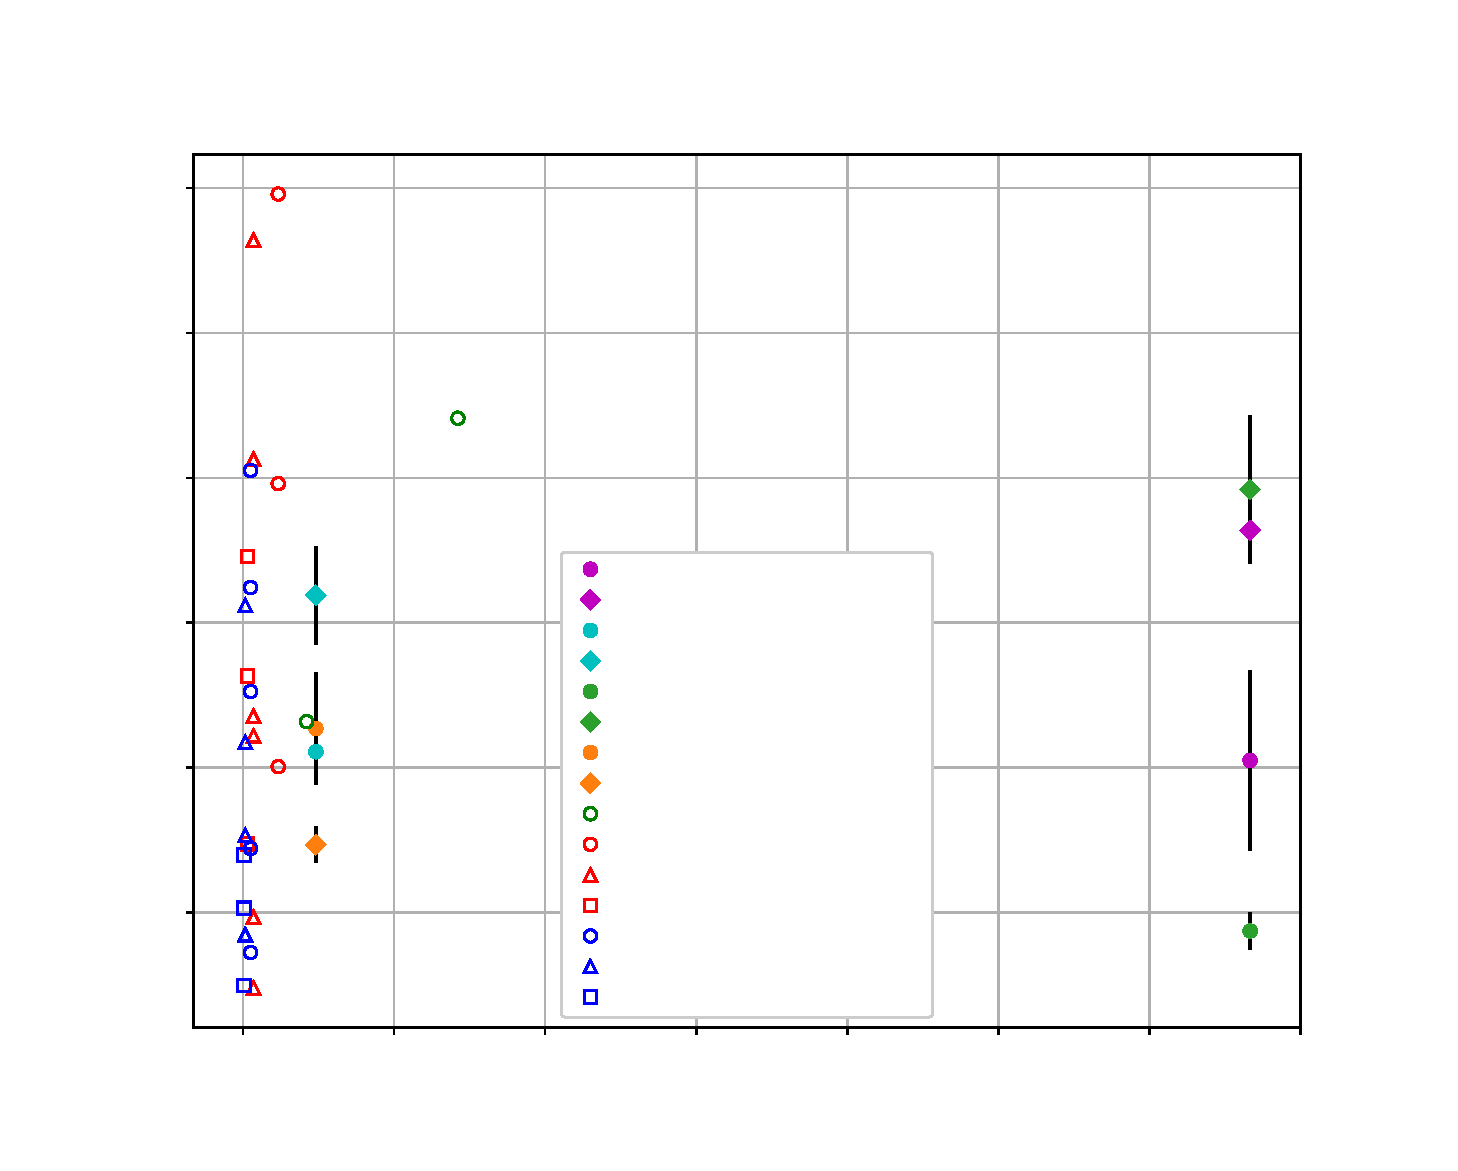
\includegraphics[width=\unitlength]{images_2ddl/expb2.eps}}%
    \put(0.15,0.05){\color[rgb]{0,0,0}\makebox(0,0)[lb]{\smash{0}}}%
    \put(0.24,0.05){\color[rgb]{0,0,0}\makebox(0,0)[lb]{\smash{50}}}%
    \put(0.34,0.05){\color[rgb]{0,0,0}\makebox(0,0)[lb]{\smash{100}}}%
    \put(0.45,0.05){\color[rgb]{0,0,0}\makebox(0,0)[lb]{\smash{150}}}%
    \put(0.55,0.05){\color[rgb]{0,0,0}\makebox(0,0)[lb]{\smash{200}}}%
    \put(0.66,0.05){\color[rgb]{0,0,0}\makebox(0,0)[lb]{\smash{250}}}%
    \put(0.77,0.05){\color[rgb]{0,0,0}\makebox(0,0)[lb]{\smash{300}}}%
    \put(0.87,0.05){\color[rgb]{0,0,0}\makebox(0,0)[lb]{\smash{350}}}%
    \put(0.045,0.1626435){\color[rgb]{0,0,0}\makebox(0,0)[lb]{\smash{0.02}}}%
    \put(0.045,0.26432625){\color[rgb]{0,0,0}\makebox(0,0)[lb]{\smash{0.04}}}%
    \put(0.045,0.366009){\color[rgb]{0,0,0}\makebox(0,0)[lb]{\smash{0.06}}}%
    \put(0.045,0.46769175){\color[rgb]{0,0,0}\makebox(0,0)[lb]{\smash{0.08}}}%
    \put(0.045,0.5693745){\color[rgb]{0,0,0}\makebox(0,0)[lb]{\smash{0.10}}}%
    \put(0.045,0.67105725){\color[rgb]{0,0,0}\makebox(0,0)[lb]{\smash{0.12}}}%
    \put(0.02,0.3573204){\color[rgb]{0,0,0}\rotatebox{90}{\makebox(0,0)[lb]{\smash{$H_{max} (m)$}}}}%
    \put(0.46293275,0.0){\color[rgb]{0,0,0}\makebox(0,0)[lb]{\smash{$k (N/m)$}}}%
    \put(0.415,0.40403532){\color[rgb]{0,0,0}\makebox(0,0)[lb]{\smash{\tiny PLA (50,5,2,34g)}}}%
    \put(0.415,0.38258502){\color[rgb]{0,0,0}\makebox(0,0)[lb]{\smash{\tiny PLA (50,5,2,64g)}}}%
    \put(0.415,0.36113473){\color[rgb]{0,0,0}\makebox(0,0)[lb]{\smash{\tiny PLA (60,5,1,12g)}}}%
    \put(0.415,0.33968444){\color[rgb]{0,0,0}\makebox(0,0)[lb]{\smash{\tiny PLA (60,5,1,17g)}}}%
    \put(0.415,0.31823415){\color[rgb]{0,0,0}\makebox(0,0)[lb]{\smash{\tiny PLA (50,4,2,34g)}}}%
    \put(0.415,0.29678385){\color[rgb]{0,0,0}\makebox(0,0)[lb]{\smash{\tiny PLA (50,4,2,64g)}}}%
    \put(0.415,0.27533356){\color[rgb]{0,0,0}\makebox(0,0)[lb]{\smash{\tiny PLA (60,8,1,17g)}}}%
    \put(0.415,0.25388327){\color[rgb]{0,0,0}\makebox(0,0)[lb]{\smash{\tiny PLA (60,8,1,20g)}}}%
    \put(0.415,0.23243444){\color[rgb]{0,0,0}\makebox(0,0)[lb]{\smash{\tiny Y&K acier (120,30)}}}%
    \put(0.415,0.21098415){\color[rgb]{0,0,0}\makebox(0,0)[lb]{\smash{\tiny Y&K polyimide (125,10)}}}%
    \put(0.415,0.18953385){\color[rgb]{0,0,0}\makebox(0,0)[lb]{\smash{\tiny Y&K polyimide (125,15)}}}%
    \put(0.415,0.16808356){\color[rgb]{0,0,0}\makebox(0,0)[lb]{\smash{\tiny Y&K polyimide (125,20)}}}%
    \put(0.415,0.14663327){\color[rgb]{0,0,0}\makebox(0,0)[lb]{\smash{\tiny Y&K polyimide (75,10)}}}%
    \put(0.415,0.12518327){\color[rgb]{0,0,0}\makebox(0,0)[lb]{\smash{\tiny Y&K polyimide (75,15)}}}%
    \put(0.415,0.10373327){\color[rgb]{0,0,0}\makebox(0,0)[lb]{\smash{\tiny Y&K polyimide (75,25)}}}%
  \end{picture}%
\endgroup%
